
%*******************************************
\section{Approach for Our Anti-Phishing Education App}
%*******************************************
\label{s:approach}
This chapter presents our final approach for the Anti-Phishing Education App.
 In the following sections we will elaborate on the app design in detail.

%===========================================
\subsection{App Design}
%===========================================
\label{s:app_design}
We have decided to divide our education app into two main parts.
 The first part of the education app is intended to increase the user awareness.
 The second part of the app then covers the actual educational part.
 The following enumeration summarizes the functions of our twofold app structure.

\begin{enumerate}
	\item \textbf{Awareness Part} The first part of the education app is intended to increase the user awareness regarding how easy it is to spoof e-mails and mislead users with such fake messages.
 This part is supposed to motivate the user to do something to counter the danger of the Internet, in this particular case, against phishing.

\begin{enumerate}
		\item \textbf{Receive Fake E-Mail} We want to illustrate to the user how easy it is to spoof the ``from'' field of an e-mail as well as the content of this e-mail.
 For this purpose the user has to send a fake e-mail with an arbitrary sender address of his choice to himself.
 The user will also have the option to type in a free text.
 Upon submitting the form the user will receive an e-mail with the e-mail address he had indicated as sender.
 The free text will also be part of the received e-mail.
 We believe that the user will be very surprised about how easy even he himself could send a fake e-mail.
 The user will learn that he cannot fully trust the ``from'' field and the content of the e-mails he is receiving.

		\item \textbf{Linktext Unequal Target URL} The awareness part of the app is also supposed to show the user that he cannot trust the texts of a link he is clicking on.
 To illustrate this, the user is asked to click on a link with the text ``https://www.
google.
de/''. Clicking on this link, the user will expect to land on the Google website, what will not happen.
 In fact, the user is linked back to our app, where he is told that link texts are not trustful as well.
 
	\item \textbf{Fake Website} Finally, the user is told that creating a copy of a website is also very easy.
 He is told that a reliable way to decide whether a website is a fake or not is to analyze the URL of the website he is visiting.
 He is also told that this app focuses on exactly this.

\end{enumerate}
	\item \textbf{Educational Part} The second part of the app covers the actual educational part.
 Here, the user is learning about various spoofing techniques of the attacker.

\begin{enumerate}
	\item \textbf{Information Material} The second part of the app is divided into levels of increasing difficulty.
 Here the user is first taught how to access and analyze the URL of the web browser.
 Subsequently, the user learns about the general structure of a URL.
 This is done in a very simplified way, so that even unexperienced users can follow.
 In particular, the user is told how to find the second- and top-level domain of a URL.
 In all succeeding levels the user is introduced to various URL spoofing techniques of a phisher.
 The learning content of each level can be consulted in~Section~\ref{s:knowledgetransferperlevel}.
		\item \textbf{Exercise to Information Material} After every introductory material in each level an exercise section is followed.
 For the ``access and analyze URL part'', for example, the user is forwarded to a website.
 There he has to apply all important steps he has learnt in the introductory part.
 After successful completion of the tasks the user is linked back to the app.
 For the ``find second- and top-level domain'' information material the user gets a couple of valid URLs of which he has to identify the second- and top-level domains.
 All subsequent level exercises are structured as follows: the user is presented a URL.
 He has to decide whether the presented URL is a phish or a valid URL.
 If the URL is a phish, and the user has correctly identified the phish, the user has to show the second- and top-level domain.
 Only if the user correctly identifies the second- and top-level domain he receives the points for this URL, otherwise the answer to this URL is considered wrong, because we assume that the user has just guessed in this case.

		\item \textbf{Repeat 2.a and 2.b With Increasing Difficulty} There is an increase of difficulty in each level.
 That is to say, in each level it gets more difficult to distinguish phishing URLs from valid ones, cf.
~Section~\ref{s:knowledgetransferperlevel}.
\end{enumerate}
\end{enumerate}

The next section deals with the concrete rules of the game.

%===========================================
\subsection{Gamification}
%===========================================
User motivation

\begin{description}
	\item[Show Leaderboard Rate]
	\item[Show Leaderboard Total]
	\item[...]
	\item[Leveling]
\end{description}

%===========================================
\subsection{Pilot Study}
%===========================================
%===========================================
\subsection{Game Rules}
%===========================================
The educational part of the app which is followed by the awareness part is divided into several levels.
 In each level the user is provided with specific informational material.
 After the information material is consulted by the user, he has to finish the according exercise.
The first  and second information materials (introduction 2 and level 1) and exercises that the user receives differ from the ones of the other levels. Here, the users obtain basic knowledge in order to bring them to the same knowledge level for the actual game.
 
\begin{description}[leftmargin=0cm]
	\item[Basic Knowledge]  The first information material and task of the user deals with accessing the address bar of a webbrowser and viewing its URL completetely.
 To prove that the user has understood how to access the address bar and view the URL he has to do the following: When the user is forwarded to the website to solve the task he has to scroll up to the top of the website to make the generally hidden address bar visible.
 Afterwards, he has to provide us the information we request about the URL in the address bar.
 This will show that he has in fact viewed the whole URL.
 After successful completion the user is linked back to the app and level 1 is started.
 From this level on, the user has three lives upon start of each level.
 In level 1 he has to identify the ``Who-Section'' (second- and top-level domain) of a URL.
 He has to tap the according part of the displayed URL.
 In this level wrong answers result in losing points and losing a live.
 In order not to frustrate the user he cannot get less than 0 points.
 When the user has no more lives left he has to restart the level.
 With every correct answer the user gains points.
	\item{Start of Actual Game}  In level 2 we start introducing URL spoofing techniques and the user has to decide whether a given URL is a phishing URL or a valid one.
 Here also, the user can lose and win points as well as lose lives.
 Here again, if the user has no more lives left he has to restart the level.
 The following Figure~\ref{fig:lose_points_life} illustrates the game flow and consequences of wrong and correct answers from level 2 and upwards.
 If the user has correctly decided that a phishing URL is a phish, he has to show us the ``Who-Section'' to prove that he has understood the concept.
 In all other cases the user is directly shown the result of his answer.
 In summary, the user looses points for any wrong answer, but he does not lose a life for every wrong answer.
 We have decided that rejecting valid URLs is not as severe as accepting phishing URLs.
 For this reason the punishment for accepting a phishing URL is more severe than the punishment for rejecting a valid URL.
 All in all, the user loses points and a live in the following cases: the user has falsely accepted a phishing URL or the user has correctly rejected a phishing URL, but could not show us the ``Who-Section''. In all other cases the user cannot lose lives, but only points.
\end{description}
 
\newline\newline
The following section deals with our leveling strategy.

\begin{figure}[hHtbp]
\centering
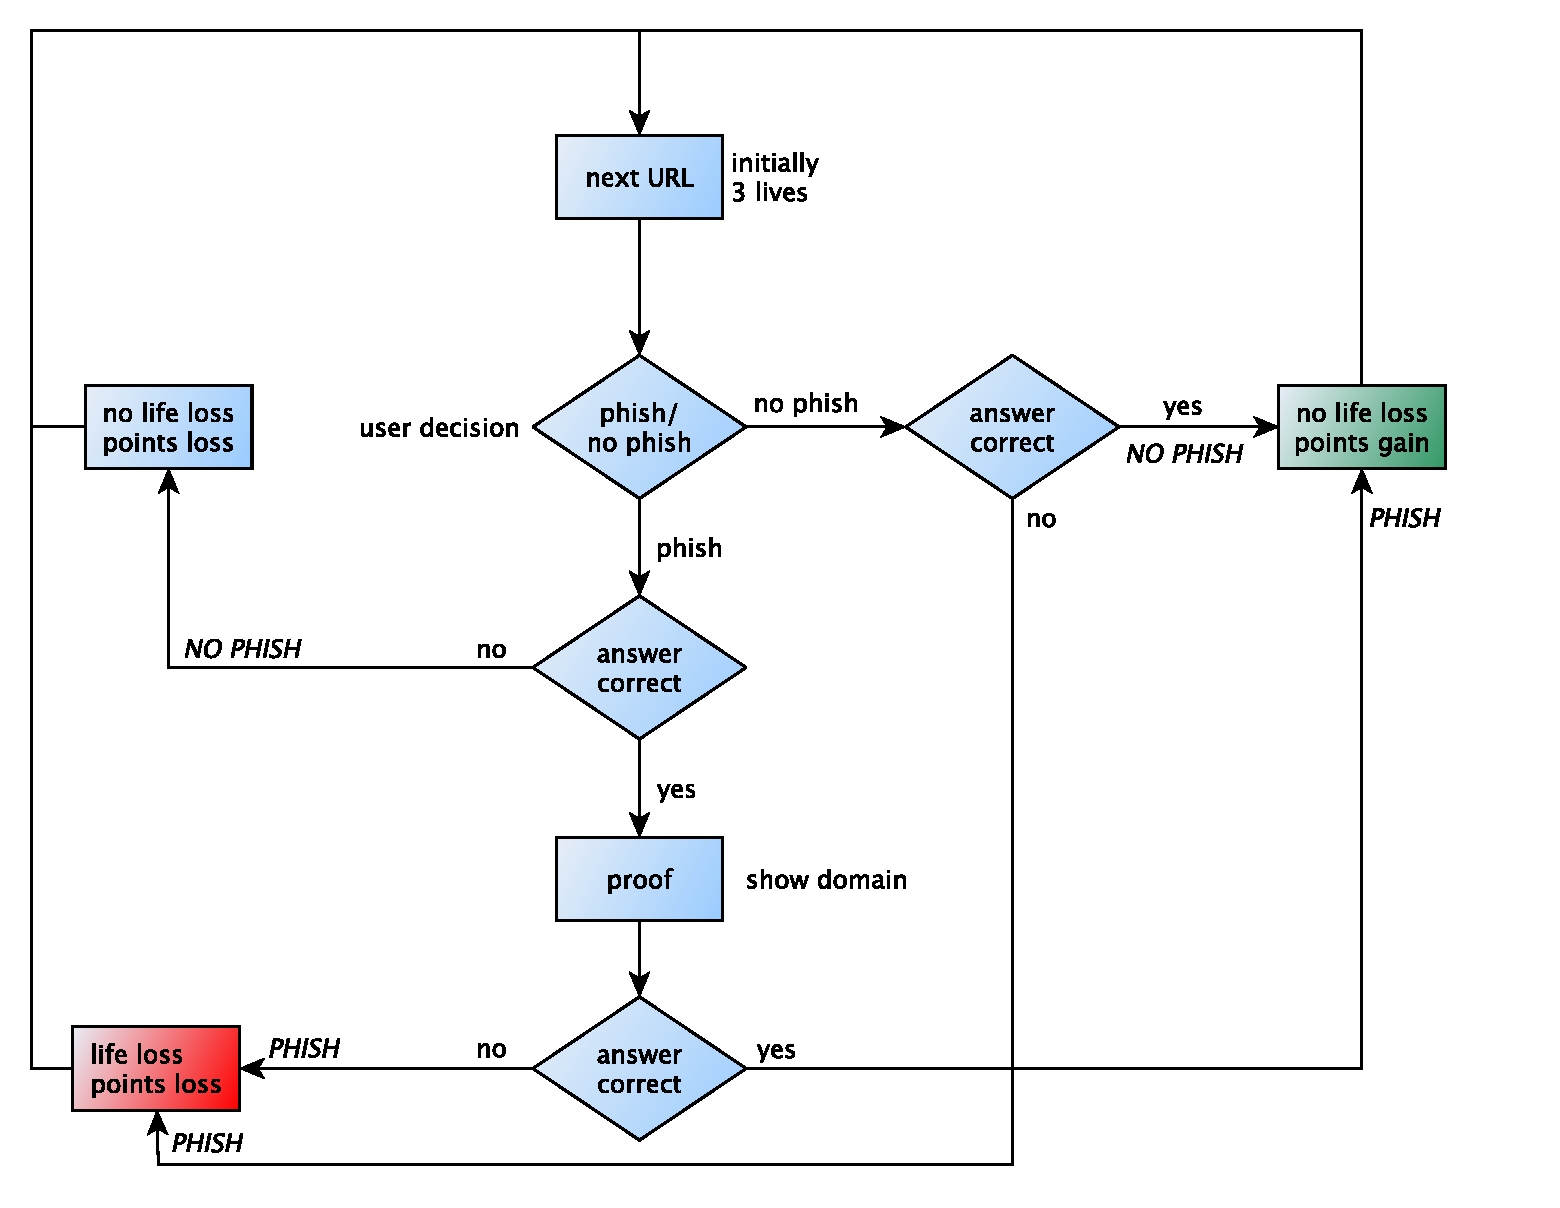
\includegraphics[width=1.0\textwidth]{graphix/lose_win_points.pdf}
\caption{Losing points and lives in the game}
\label{fig:lose_points_life}
\end{figure}
%===========================================
\subsection{Leveling Strategy}
%===========================================
During the app development we have tried out several leveling strategies.
 This section is intended to introduce the leveling strategies we have considered for the app.


\begin{description}[leftmargin=0cm]
	\item[Leveling Based on Achieved Points] Our very first leveling strategy was based on the achieved points per level.
 Each level the user had to achieve at least 100 points to pass the current level and unlock the next one.
 This approach had a major drawback.
 The fact that achieving a minimum of points to pass the level resulted in very similar points for everybody finishing a level.
 That is to say, everybody who has finished level x, has approximately the same points, which in turn would have meant that the comparison between single users would not be meaningful as it would only differ very slightly.
 Additionally, with this strategy, users might replay early levels which are easier and gain the same amount of points as users playing later levels.
 This might result in users playing early levels repeatedly get more points than users playing later and difficult levels.

	\item[Leveling Based on Detected Phishes] The previously described leveling strategy had the deficit of comparability among the users.
 However, we consider comparability very important  since it serves as an incentive for the user to play better or play on.
 For this reason we overthought our strategy and decided that passing a level should not depend on the points a user receives.
 It rather should depend on the number of phishes the user was able to detect during a level.
 That is to say, among the shown URLs in every level there is a certain amount of phishes the user has to detect in order to pass the level.
 With this approach however, there is still the possibility for a user to repeat early, and thus easy, levels and possibly gain more points than users playing later, and thus more difficult, levels.
 To prohibit this, in increasing levels the users gains and loses increasing points accordingly.
 In this way, a user repeating early levels is not able to catch up other users of higher levels.
 This strategy solved the problems of our first strategy, however it also brought a new one.
 The strategy of passing the level when a certain amount of phishes are detected has the following flaw: always rejecting a URL will eventually result in passing the level (if the user also correctly identifies the ``Who-Section'' when required). The user will not gain a lot of points with this strategy, however he will eventually win, which is suboptimal for a game.
  
	\item[Leveling Based on Correct Answers] To solve the problem of our second leveling approach we have extended the leveling passing to correct answers.
 Instead of detecting a certain amount of phishes per level, the user has to give correct answers to a predefined amount of phishing URLs as well as a predefined amount of valid URLs in order to pass the level.
 Only and only if the user has answered the predefined number of valid and phishing URLs the level is completed.
 To additionally incentivize the users we have included three lives per level.
 The lives are supposed to prevent a user playing eternally, without ever passing the current level.
 When the user loses all of his lives, cf.
~Figure~\ref{fig:lose_points_life}, this is an indication that he did not understand what the level is about.
 Consequently, he has to restart the level by being forwarded to the introductory part of the current level.
 This is our final leveling strategy for the app.

\end{description}


%===========================================
\subsection{Teaching Goals Per Level}
%===========================================
\label{s:knowledgetransferperlevel}
This section summarizes the learning objectives of each level.
 Note that we generally do not use technical term like URL, domain, subdomain, protocol or the like.


\begin{description}[leftmargin=0cm]
	\item[Introduction 1] This part is the awareness part described in Section~\ref{s:app_design}. Here, the user learns how easy e-mail spoofing is.
 Additionally, the user is informed about the simplicity of setting up fake websites and that he should not trust the texts of the links he is clicking on.

	\item[Introduction 2] In this part the user is explained how he can access the URL of a web browser and how exactly he has to look at the whole URL.
 In particular, the user is told that he has to scroll up the whole website to make the generally hidden address bar re-appear.
 Then he has to tap the text field of the address bar and scroll to the start of the URL.
 At the end of the exercise for this the user is told that he always has to analyze the URL like this, because all other displayed URLs or links might be fake too.

	\item[Level 1] The actual game starts with level 1, where the user learns about the structure of a URL.
 First of all, the user gets an overview of the single components of a URL.
 To make the comprehension of these components easier to understand we used an analogy which is summarized in Figure~\ref{fig:url_components} with an example URL.
 We told the user that he has to imagine that the website he is visiting is his dialog partner.
 The user is told that the section between ``http(s)://'' and the third slash ``/'', i.
e.
 the hostname, reveals information about his dialog partner.
 In particular, we explain that he has to read this part from right to left.
 The top-level and second-level domain is introduced as ``Who-Section'' (company + location of company), from which the user knows who he is actually talking to.
 All succeeding parts in this area are to be considered as ``departments'' of the company of ther user's dialog partner.
 The protocol part is introduced as ``Security Level'' of the dialog with the partner and the path part of a URL, i.
e.
 the part after the third slash ``/'', is introduced as the topic of the conversation with the dialog partner.
 When marking parts of a URL we consistently used the according colour of Figure~\ref{fig:url_components}. The main objective of the level 1 exercise is to be able to identify the second- and top-level domain of a URL.

	\item[Level 2] With level two we start introducing the spoofing tricks of a phisher.
 We considered the subdomain attack, cf.
~Section~\ref{s:url_categories}, as a good starting point to introduce the phisher as the user has just learnt about the importance of the ``Who-Section'' (top-level and second-level domain) in level 1.
	\item[Level 3] In level 3 the user is first told what an IP address is.
 To facilitate the comprehensibility, we used the analogy of house addresses.
 The user is explained that like addressing our houses with street names and numbers, computers in the Internet are addressed by so called IP addresses.
 The IP address itself is defined as a 4-place sequence of numbers, separated by dots.
 Finally, the user is warned against URLs with IP addresses in the host part.

	\item[Level 4] In this level we deal with nonsense in the second-level domain, cf.
~Section~\ref{s:url_categories}.
	\item[Level 5] In this level we deal with second-level domain names which sound trustworthy, but are in fact unrelated to the company name, cf.
~Section~\ref{s:url_categories}.
	\item[Level 6] Here misleading and deceiving names in the second-level domain of a URL are covered.
 This includes typos, scrambled letters or other similar and deceptive names in the second-level domain, cf.
~Section~\ref{s:url_categories}.
	\item[Level 7] In this level we focus on homographic attacks, where the user is able to visually distinguish a fake second-level domain from the original one, cf.
~Section~\ref{s:url_categories}.
	\item[Level 8] In this level the user is introduced to an attack where the brand name of the visited website or even the whole legitimate URL is placed in the path of a fake URL, cf.
~Section~\ref{s:url_categories}.
	\item[Level 9] Here we introduce the difference between the usage of http:// and https://. In particular, the user is told that the usage of https:// means that his conversation with the website is encrypted and that the dialog partner indicated in the ``Who-Section'' is authenticated.
 As an analogy we say that the https:// represents a higher security level.
 This means, the conversation cannot be eavesdroppbed by a third party and the dialog partner indictated in the ``Who-Section'' has proved his identity to a trusted third party.
 With http:// this security level is not established.

	\item[Level 10] This level does not include an exercise.
 It mainly serves as a section with some important additional input for the user.
 Specifically, we tell the user two things: First, we explain to him that he might encounter URLs which actually look very phishy.
 In such a case, we suggest him to directly contact the company and ask for the authenticity of the specific website.
 Furthermore, we introduce extended validation certificates.
 We provide the user with a link to further information to this subject.

\end{description}

\begin{figure}[hHtbp]
\centering
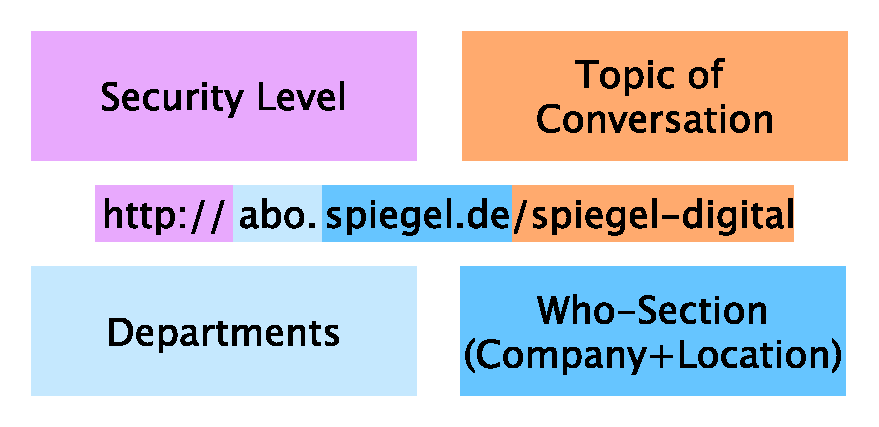
\includegraphics[width=0.56\textwidth]{graphix/url_components.pdf}
\caption{URL components that are communicated to the user}
\label{fig:url_components}
\end{figure}
%===========================================
\subsection{URL Generation}
%===========================================


